\documentclass[aspectratio=169, 11pt]{beamer}
\usepackage[utf8]{inputenc}
\usepackage[T1]{fontenc}
\usepackage{amsmath}
\usepackage{hyperref}
\usepackage{xcolor}
\usepackage{multicol}
\usepackage{graphicx}

% Set the theme
\usetheme{Warsaw}

% Set the color theme
\usecolortheme{orchid}

% Set the font theme
\usefonttheme{default}

% Define a custom color
\definecolor{myblue}{RGB}{33, 66, 99}
\definecolor{lightblue}{RGB}{80, 133, 244}
\setbeamercolor{structure}{fg=lightblue}

% Use sans serif font as default
\renewcommand{\familydefault}{\sfdefault}

% Change background color
\setbeamercolor{background canvas}{bg=white}

% Title page
\title[Sound Detection and Classification]{\textbf{Sound Detection and Classification}\\ using Spiking Neural Networks}
\author[T. Courrege, L. Gandeel]{Téo Courrege\\Loaï Gandeel}
\date{\today}


% Customize title page
\setbeamertemplate{title page}{
  \begin{centering}
    \vfill
    \textcolor{myblue}{\LARGE\inserttitle}\par
    \vspace{1cm}
    \textcolor{black}{\large\insertauthor}\par
    \vspace{1cm}
    \textcolor{black}{\small\insertdate}\par
    \vfill
  \end{centering}
}

% Customize section page
\AtBeginSection[]{
  \begin{frame}{Outline}
    \begin{multicols}{2}
      \hfill % This will push the table of contents to the right side
      \tableofcontents[currentsection, sectionstyle=show/shaded, subsectionstyle=show/show/hide]
    \end{multicols}
  \end{frame}
}


\begin{document}

\begin{frame}[plain]
  \titlepage
\end{frame}

\section{Introduction}


\section{Theoretical Study}

\subsection{Theoretical Study of SNN}

\begin{frame}
  \frametitle{Comparison: ANN vs SNN}
  \begin{columns}
    \begin{column}{0.5\textwidth}
      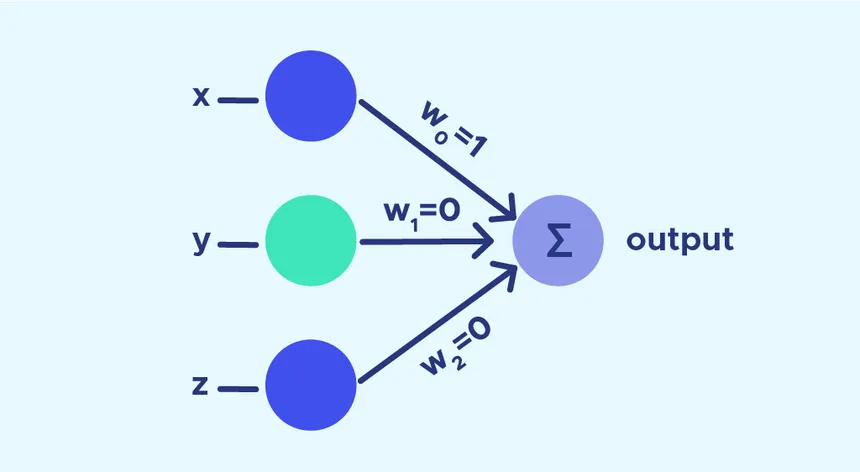
\includegraphics[width=\textwidth]{image/perceptrons.png}
    \end{column}
    \begin{column}{0.5\textwidth}
      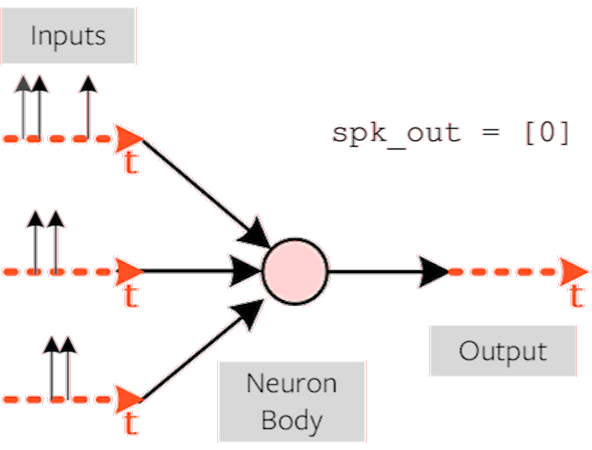
\includegraphics[width=\textwidth]{image/def1.png}
    \end{column}
  \end{columns}
\end{frame}

\begin{frame}
  \frametitle{Specificities of SNNs}
  \begin{itemize}
    \item Neurons communicates with each other by sending spikes.
    \item More biologically realistic than ANNs.
    \item More energy efficient than ANNs (real time processing, event driven processing, sparse representation).
    \item Loss function is not differentiable and cannot be optimized using gradient descent for backpropagation.
  \end{itemize}
\end{frame}

\begin{frame}
  \frametitle{Comparison between spiking neural models}
  \begin{center}
    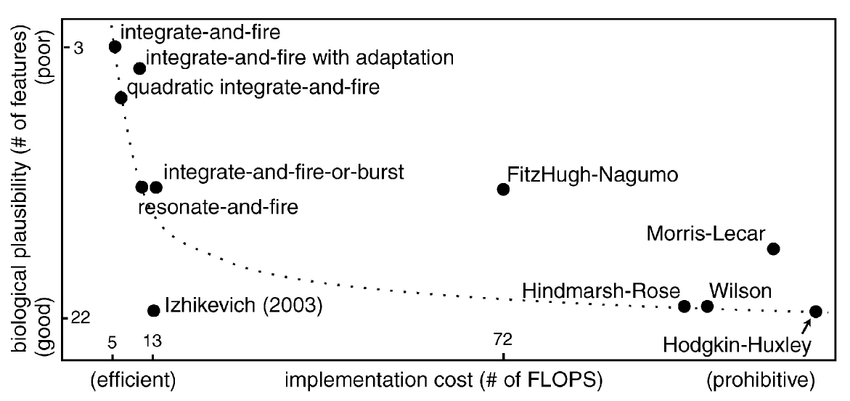
\includegraphics[width=0.8\textwidth]{image/theo1.png}
  \end{center}
\end{frame}

\subsection{LIF Model}
\begin{frame}
  \frametitle{Principle of LIF}
  \begin{columns}
    \begin{column}{0.5\textwidth}
      \begin{itemize}
        \item Leaky integrate-and-fire in SNNs:
        \item Accumulates input currents over time
        \item Leaking a fraction of the charge per unit time
        \item Fires when the accumulated charge surpasses a threshold.
      \end{itemize}
    \end{column}
    \begin{column}{0.5\textwidth}
      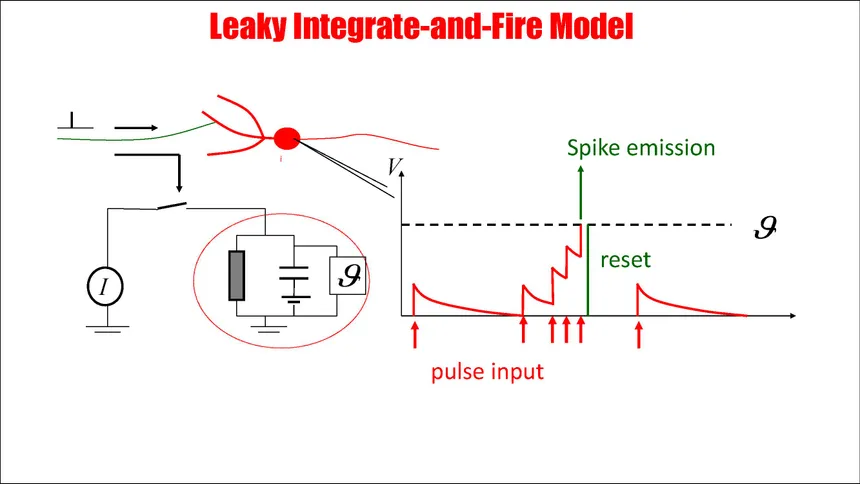
\includegraphics[width=\textwidth]{image/lif.png}
    \end{column}
  \end{columns}
\end{frame}

\begin{frame}
  \frametitle{LIF Model Equations}
  $$ C_m \frac{d V_m}{d t} = I(t) - \frac{V_m}{R_m} $$
  \begin{itemize}
    \item $C_m$ is the membrane capacitance
    \item $V_m$ is the membrane potential
    \item $I(t)$ is the input current
    \item $R_m$ is the membrane resistance
  \end{itemize}
\end{frame}

\section{Data, Objectives and State of the Art}

\subsection{Data}

\begin{frame}{Choosing the Type of Training Data}
  \begin{itemize}
    \item Understanding the challenges of training SNNs compared to ANNs.
    \item Criteria for selecting data: Less computationally intensive, adaptable to pre-recorded and real-time processing.
  \end{itemize}
\end{frame}

\subsection{Objective}

\begin{frame}{Feasibility}
  \begin{itemize}
    \item Selection of Google AudioSet database.
    \item Addressing copyright concerns (Creative Commons license).
    \item Data collection/extraction: Utilizing GitHub repositories for efficient downloading, formatting, and cropping of sound files.
    \item Assessing resource usage and parallelization impact.
    \item Uncertainties about data quality: Contextual issues, multi-labeling, Weak and Strong Label annotations.
  \end{itemize}
\end{frame}

%Technical Objectives Achievable with Pre-existing ANNs


\subsection{Feasibility}

\begin{frame}{Feasibility}
  \begin{itemize}
    \item Addressing uncertainties related to dynamic audio signals, varying acoustic environments, and challenges in modeling temporal aspects.
    \item Discussing potential challenges in training SNNs, considering non-linearity and sparsity of spikes.
    \item Highlighting potential data uncertainties, such as varied audio formats and unavailability of certain samples.
    \item Estimating computation time for data import and training.
  \end{itemize}
\end{frame}

\subsection{State of the Art}

\begin{frame}{ANNs Used for Audio Classification}
  \begin{itemize}
    \item Overview of existing ANNs for audio classification.
    \item Mentioning pre-trained models on Google AudioSet, rearranged Resnet, inception, densenet, and LSTM-based models.
    \item Providing references to relevant GitHub repositories and research papers.
  \end{itemize}
\end{frame}

\begin{frame}{SNNs Used for Audio Classification}
  \begin{itemize}
    \item Overview of existing SNNs for audio classification.
    \item Highlighting spiking convolutional neural networks (SCNN), multi-layer SNN using SpiNNaker, shadow training, and SNN simulators (BindsNET, NEST).
    \item Referencing GitHub repositories and documentation for each model.
  \end{itemize}
\end{frame}

\subsection{Pre-processing}
\begin{frame}{Pre-processing}
  \begin{itemize}
    \item Collecting the data
    \item Adaptation of the data
    \item Checking that there are no errors / repetitions
  \end{itemize}
\end{frame}

\section{Spectrograms, MEL and MFCC}
\subsection{Spectrograms}

\begin{frame}{Spectrograms}
  \begin{itemize}
    \item Spectrograms
  \end{itemize}
\end{frame}

\subsection{MEL}

\begin{frame}{MEL}
  \begin{itemize}
    \item MEL
  \end{itemize}
\end{frame}

\subsection{MFCC}

\begin{frame}{MFCC}
  \begin{itemize}
    \item MFCC
  \end{itemize}
\end{frame}

\section{Spiking Neural Networks - First results}

\begin{frame}{Spiking Neural Networks - First results}
  \begin{itemize}
    \item First results
  \end{itemize}
\end{frame}

\section{Conclusion}

\begin{frame}{Conclusion}
  \begin{itemize}
    \item Summary
    \item Future Work
  \end{itemize}
\end{frame}

\end{document}
